\documentclass{article}
\usepackage[utf8]{inputenc}
\usepackage[french]{babel}
\usepackage[T1]{fontenc}
\usepackage{fullpage}
\usepackage{amsmath}
\usepackage{amssymb}
\usepackage{graphicx}
\usepackage{enumitem}
\usepackage{subfig}
\usepackage{hyperref}
\usepackage{color}
\usepackage[table]{xcolor}
\usepackage{listings}

\definecolor{darkWhite}{rgb}{0.94,0.94,0.94}
 
\lstset{
  aboveskip=3mm,
  belowskip=-2mm,
  backgroundcolor=\color{darkWhite},
  basicstyle=\footnotesize,
  breakatwhitespace=false,
  breaklines=true,
  captionpos=b,
  commentstyle=\color{red},
  deletekeywords={...},
  escapeinside={\%*}{*)},
  extendedchars=true,
  framexleftmargin=16pt,
  framextopmargin=3pt,
  framexbottommargin=6pt,
  frame=tb,
  keepspaces=true,
  keywordstyle=\color{blue},
  language=Python,
  literate=
  {²}{{\textsuperscript{2}}}1
  {⁴}{{\textsuperscript{4}}}1
  {⁶}{{\textsuperscript{6}}}1
  {⁸}{{\textsuperscript{8}}}1
  {€}{{\euro{}}}1
  {é}{{\'e}}1
  {è}{{\`{e}}}1
  {ê}{{\^{e}}}1
  {ë}{{\¨{e}}}1
  {É}{{\'{E}}}1
  {Ê}{{\^{E}}}1
  {û}{{\^{u}}}1
  {ù}{{\`{u}}}1
  {â}{{\^{a}}}1
  {à}{{\`{a}}}1
  {á}{{\'{a}}}1
  {ã}{{\~{a}}}1
  {Á}{{\'{A}}}1
  {Â}{{\^{A}}}1
  {Ã}{{\~{A}}}1
  {ç}{{\c{c}}}1
  {Ç}{{\c{C}}}1
  {õ}{{\~{o}}}1
  {ó}{{\'{o}}}1
  {ô}{{\^{o}}}1
  {Õ}{{\~{O}}}1
  {Ó}{{\'{O}}}1
  {Ô}{{\^{O}}}1
  {î}{{\^{i}}}1
  {Î}{{\^{I}}}1
  {í}{{\'{i}}}1
  {Í}{{\~{Í}}}1,
  morekeywords={*,...},
  numbers=left,
  numbersep=10pt,
  numberstyle=\tiny\color{black},
  rulecolor=\color{black},
  showspaces=false,
  showstringspaces=false,
  showtabs=false,
  stepnumber=1,
  stringstyle=\color{olive},
  tabsize=4,
  title=\lstname,
}

\begin{document}
\begin{titlepage}

\begin{center}
\newcommand{\HRule}{\rule{\linewidth}{0.5mm}}

\vspace{1cm}
\textsc{\LARGE INGInious}
\vspace{7cm}

\HRule \\[1cm]
{\huge \bfseries Création d'exercices sur INGInious\\ \vspace{0.4cm} Tutoriel\\[1cm]}
\HRule \\
\vspace{1.5cm}

\large{\emph Auteur : }\\
\vspace{0.3cm}

\textsc{Oreins} Manon\\

\vfill


\large Juillet 2020
\end{center}
\end{titlepage}

\tableofcontents
\thispagestyle{empty}
\setcounter{page}{0}
\newpage

\section{Premier pas sur INGInious}

Si vous souhaitez créer un cours, il est nécessaire de contacter l'administrateur de la plateforme. 

Plus d'informations dans la documentation officielle d'INGInious : 
\bigskip

\url{https://inginious.readthedocs.io/en/latest/index.html}

\bigskip
En étant l'administrateur d'un cours sur INGInious, l'accès à de nombreuses fonctionnalités vous est permise grâce à l'onglet "Administration du cours". 

Dans "Paramètres du cours" vous pourrez, notamment, ajouter des administrateurs et modifier l'accessibilité et les inscriptions des étudiants à ce cours. Dans la partie "Étiquettes", il est possible de créer des étiquettes à attacher aux exercices et qui permettront aux étudiants de filtrer la liste d'exercices en fonction de celles-ci, ce qui est très utile quand le cours possède un grand nombre d'exercices. Elles peuvent, par exemple, servir à indiquer un chapitre de la matière ou un niveau de difficulté. Pour vous exercer, créez une étiquette ayant comme ID "Test" et cochez la case "visible pour l'étudiant". Si vous souhaitez plus d'informations concernant les étiquettes, suivez le lien ci-dessous :
\bigskip

\url{https://dial.uclouvain.be/memoire/ucl/object/thesis:14637}
\bigskip

Ce tutoriel se penchera sur l'onglet "Exercices" qui permet de créer et d'ajouter vos propres exercices au cours. Les autres parties, bien qu'intéressantes, ne seront pas développées ici, mais n'hésitez pas à aller les découvrir par vous-même. 

\section{Création d'un exercice simple}

Nous allons maintenant créer un exercice basique qui pourra vous servir de base. Après avoir cliqué sur l'onglet "Exercices", vous arrivez ici :

\begin{figure}[h]
    \centering
    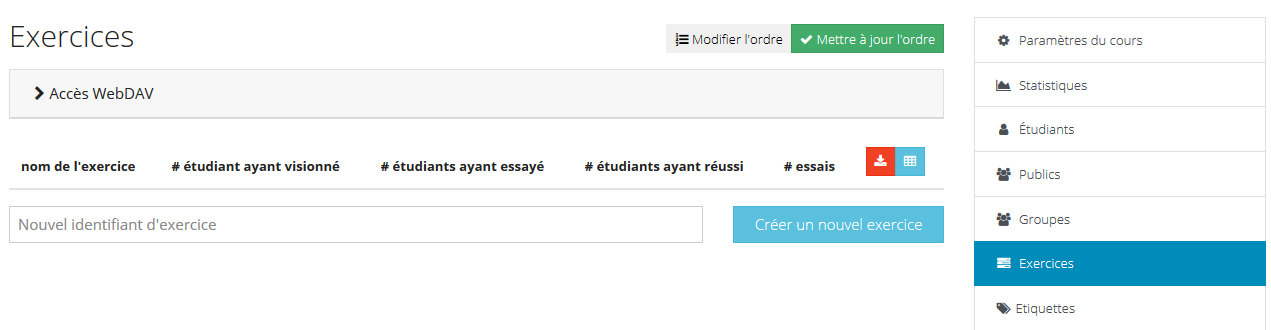
\includegraphics[scale=0.5]{images/Exercices.PNG}
\end{figure}

Après avoir choisi un identifiant, qui devra être différent pour chaque exercice, vous pouvez créer votre premier exercice.
Dans les paramètres de base vous pouvez ajouter un nom à votre exercice, c'est celui que verront les étudiants, à la différence de l'identifiant, que seuls les administrateurs peuvent voir.  L'option "Catégorie" permet d'attacher une ou plusieurs étiquettes à l'exercice. Vous pouvez également rajouter un énoncé, l'auteur et d'autres paramètres que nous n'allons pas détailler. Voici un exemple :

\begin{figure}[!htb]
    \centering
    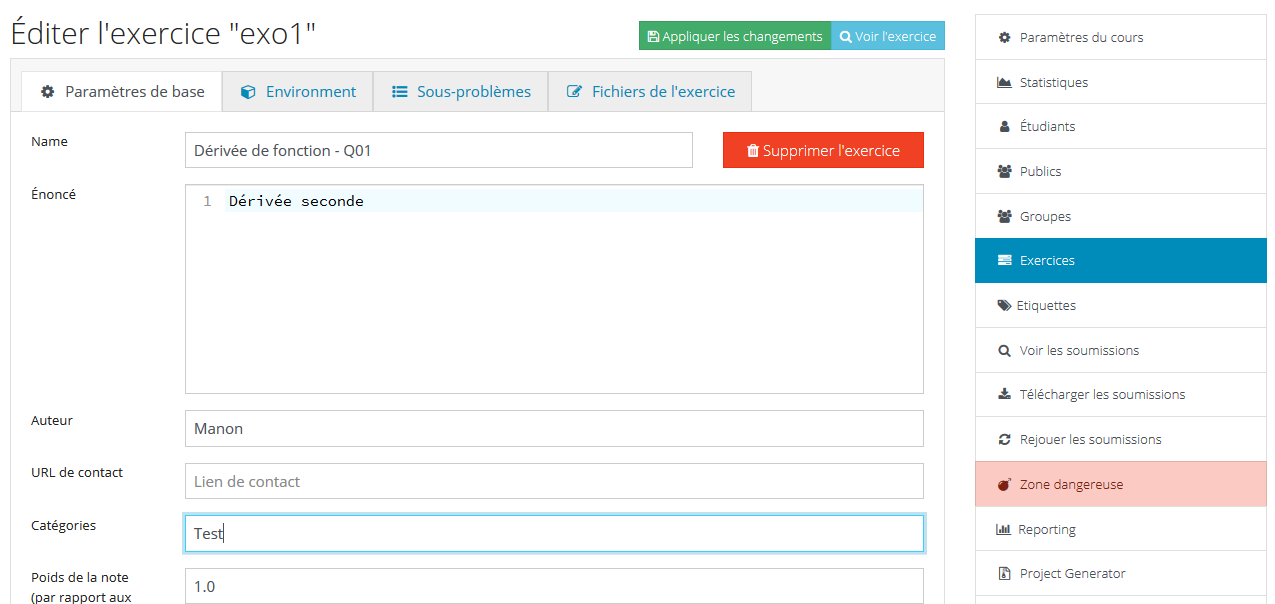
\includegraphics[scale=0.4]{images/Para.PNG}
\end{figure}

\newpage
Vous pouvez maintenant passer à l'onglet "Environment", comme nous allons réaliser un exercice assez simple, sélectionnez "Multiple Choice Question solver" dans la partie "Grading environment type". 

\begin{figure}[!htb]
    \centering
    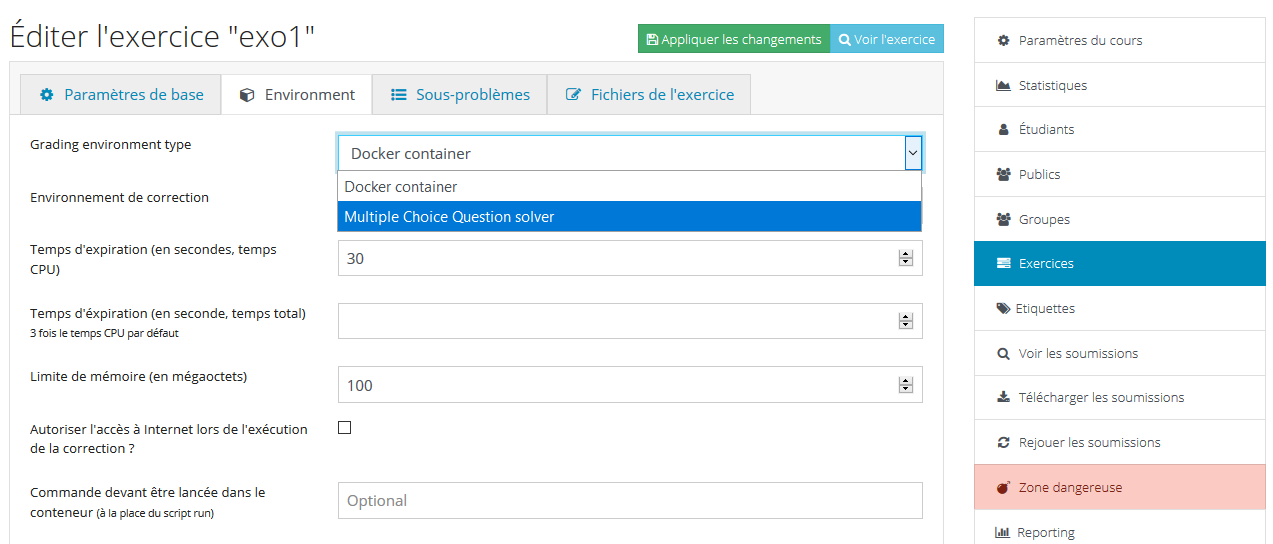
\includegraphics[scale=0.49]{images/Envi.png}
\end{figure}

Passez maintenant à l'onglet "Sous-problèmes". Vous pouvez y ajouter une ou plusieurs questions. Chaque identifiant doit être différent. Il existe plusieurs types de sous-problèmes, pour des exercices de mathématiques ce sera essentiellement "math","choix multiple" ou "code (une seule ligne)". Pour l'exemple nous allons faire une sous-question de type "math" et une autre de type "choix multiple". Après création on obtient ceci :

\begin{figure}[!htb]
    \centering
    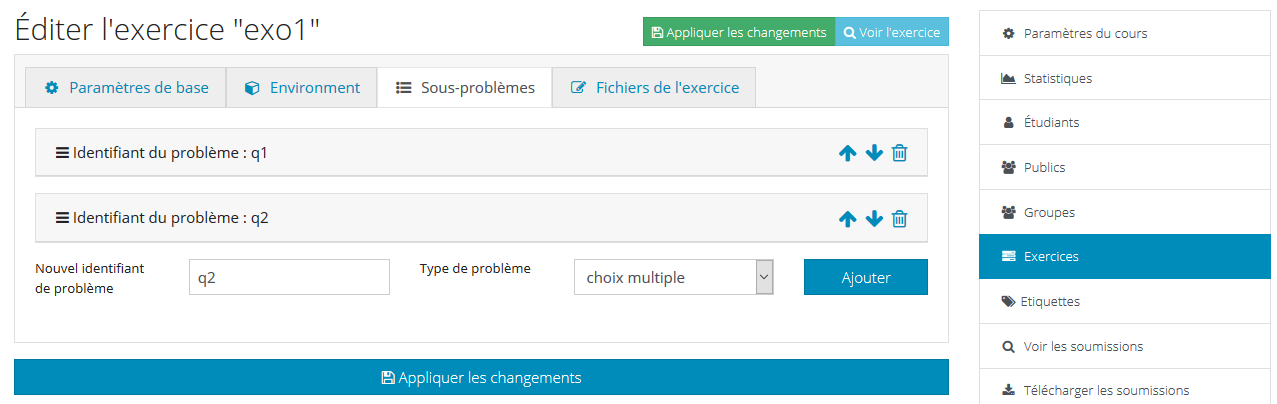
\includegraphics[scale=0.5]{images/sous_prob.png}
\end{figure}

Vous pouvez changer l'ordre des questions grâce aux flèches sur la droite.
Pour l'instant, ces questions sont vides, nous allons donc les modifier, pour cela, cliquez sur les trois barres horizontales à côté de l'identifiant du sous-problème. Vous pouvez alors rajouter un nom, l'énoncé de la sous-question, un indice que pourra voir l'étudiant et des feedbacks en cas d'échec ou de réussite. Ajoutez ensuite une ou plusieurs réponses attendues. Vous avez également la possibilité d'ajouter des "Possible wrong answers" . Elles permettent de rajouter des erreurs que pourraient faire les étudiants et de donner des feedbacks personnalisés en fonction de ces erreurs. 

Voici notre exemple :

\begin{figure}[!htb]
    \centering
    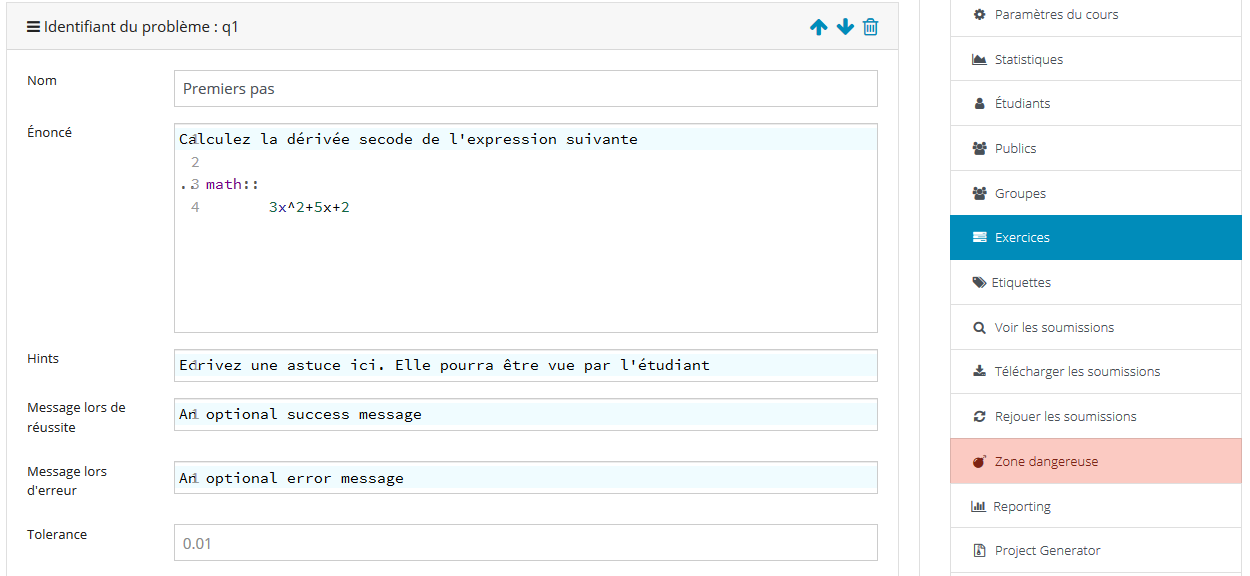
\includegraphics[scale=0.5]{images/sp.png}
\end{figure}

\begin{figure}[!htb]
    \centering
    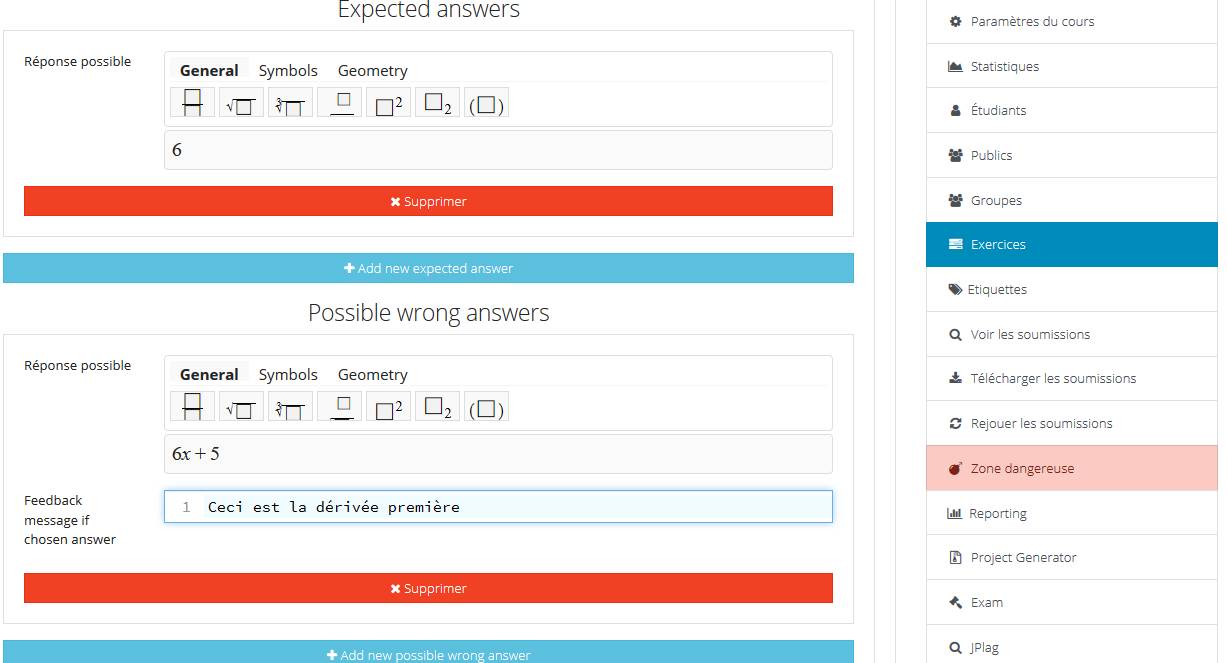
\includegraphics[scale=0.5]{images/sp1.png}
\end{figure}

\newpage
Modifions maintenant le deuxième sous-problème. Vous pouvez à nouveau rajouter un nom et un énoncé, ainsi que les choix qui composeront le qcm et des feedbacks optionnels. Appuyez sur la case "Correct ?" pour les choix qui sont corrects. N'oubliez pas de cocher la case "Réponses multiples" si c'est le cas. Les propositions sont automatiquement mélangées à chaque rafraichissement de la page, l'ordre dans lequel vous les mettez n'a donc aucune importance. 
\bigskip

Dans notre exemple nous allons mettre deux choix et une réponse correcte :

\begin{figure}[!htb]
    \centering
    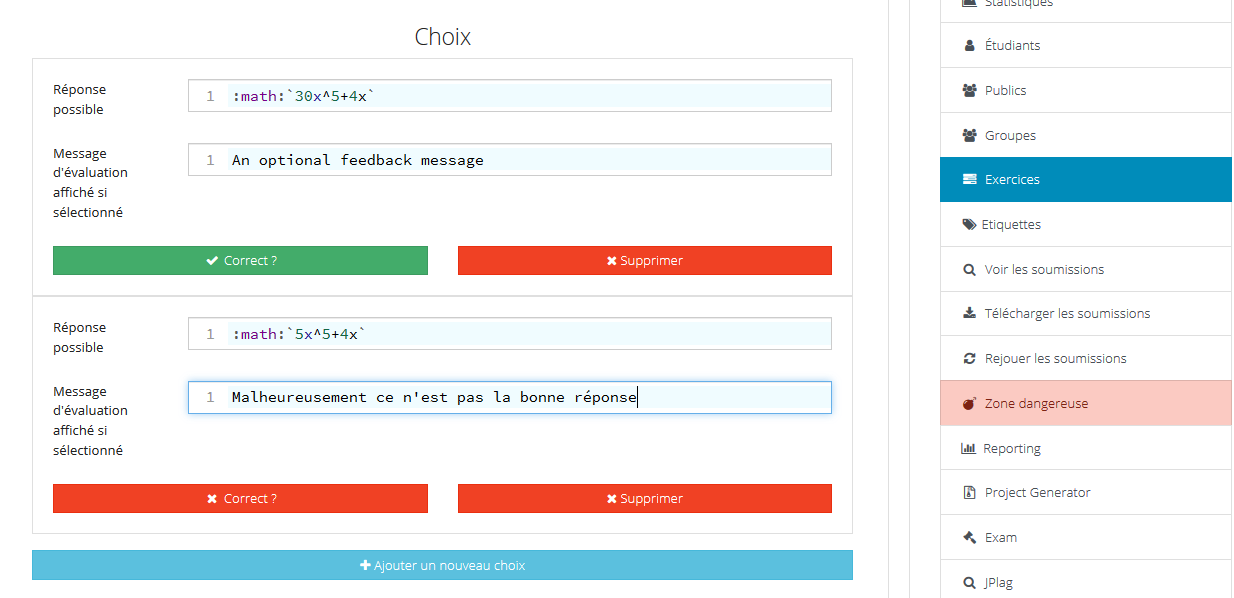
\includegraphics[scale=0.5]{images/qcm.png}
\end{figure}

\newpage
Nos sous-questions sont maintenant terminées. On ne doit pas modifier l'onglet "Fichiers de l'exercice" pour le moment, il ne nous reste donc qu'à sauvegarder les modifications en cliquant sur "Appliquer les changements" et à visualiser notre exercice.
Si vous avez bien créé l'étiquette "Test" comme mentionné au début du tutoriel, les exercices devraient s'afficher correctement comme ceci :

\begin{figure}[!htbp]
    \centering
    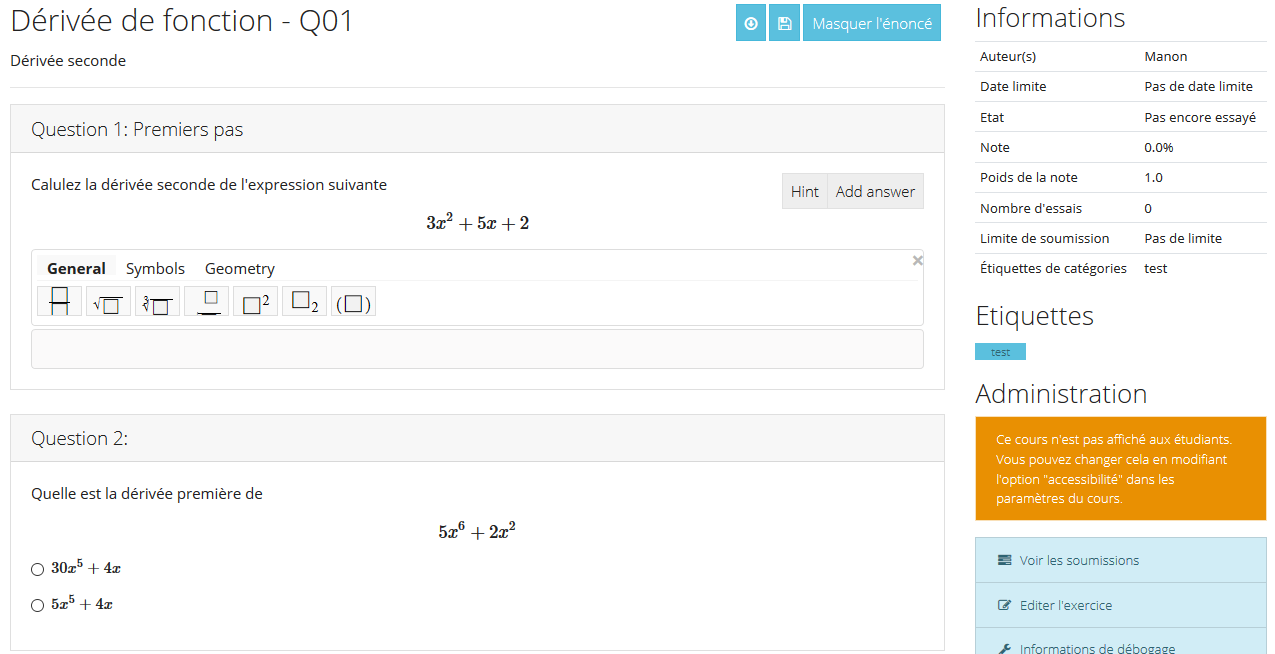
\includegraphics[scale=0.48]{images/exo_fini.png}
\end{figure}
\newpage


N'hésitez pas à entrer des différentes réponses afin de voir comment la plateforme réagit, essayez également le bouton "hint".

\bigskip
Vous avez peut être remarqué l'utilisation de formules spéciales pour l'écriture des différentes équations. Elles sont écrites en LaTeX, pour utiliser ce langage il est nécessaire d'utiliser des balises.
\bigskip

\begin{itemize}
    \item Dans le texte, exemple : :math${:}$`3x` comme dans les choix multiples de l'exemple. (Attention il faut un espace avant et après la balise)
    \item Dans un bloc, exemple :
    
    .. math${::}$
    
    \hspace{1cm} 3x+2
    
    Comme dans l'énoncé de la première question de l'exemple
\end{itemize}

Vous trouverez plus d'informations sur l'écriture des formules en LaTeX depuis le lien suivant :
\bigskip

\url{https://fr.wikibooks.org/wiki/LaTeX/Écrire_des_mathématiques}

\bigskip

Les énoncés sont écrit en reStructuredText, il est donc possible d'ajouter des tableaux, des listes d'éléments, des titres et des hyperliens. Vous pouvez trouver toutes les informations pour les réaliser en suivant ce lien :

\bigskip
\url{https://docutils.sourceforge.io/docs/user/rst/quickref.html}

\section{Création d'exercices plus complexes}

Nous allons maintenant présenter quelques types d'exercices plus complexes qui nécessitent d'ajouter un fichier comprenant du code et des paramètres différents.

\subsection{Domaine de fonction} \label{dom fct}

Cette première partie concerne les exercices demandant une réponse sous la forme d'un intervalle ([2;5]), comme un domaine de définition d'une fonction, ou d'un ensemble de point (\{1,6,8\}).
\bigskip

Quand vous créez ce type d'exercice, il est nécessaire que le "Grading environment type" dans l'onglet "Environment" soit "Docker container", ne changez donc rien dans cet onglet.
Lorsque vous créez un sous-problème, il doit être de type "code(une seule ligne)". Pour plus de facilité, nommez vos sous-problèmes "q1","q2"... Écrivez votre énoncé dans l'encadré correspondant. Il n'y a pas d'endroit où indiquer la réponse correcte et c'est tout à fait normal car nous allons l'inscrire dans un fichier.

Dans l'onglet "Fichier de l'exercice", créez un nouveau fichier que vous nommerez "run". 

\begin{figure}[!htb]
    \centering
    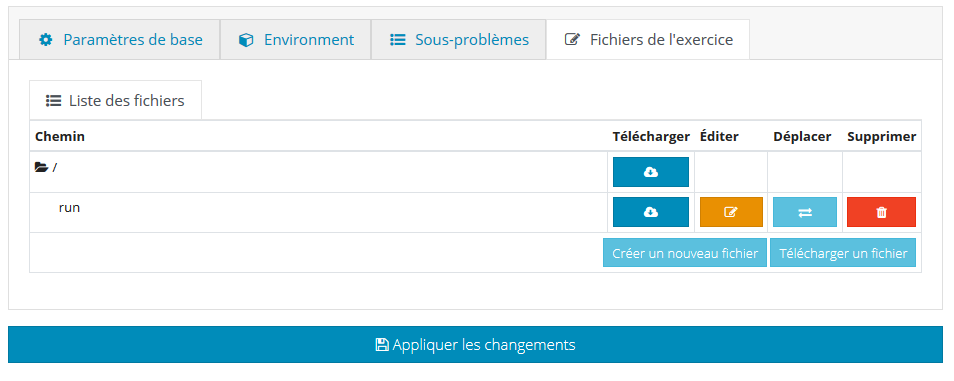
\includegraphics[scale=0.5]{images/fichier.png}
\end{figure}

Pour éditer ce fichier, appuyez sur la case orange. Ensuite, copiez-collez et modifiez en suivant les commentaires le contenu du fichier "exo\_parsingDomain.py" disponible en téléchargement via le lien ci-dessous :

\bigskip
\url{https://github.com/UCL-INGI/inginious-math/blob/master/exo_parsingDomain.py}
\bigskip.

Voici un exemple de question :

\begin{figure}[!htb]
    \centering
    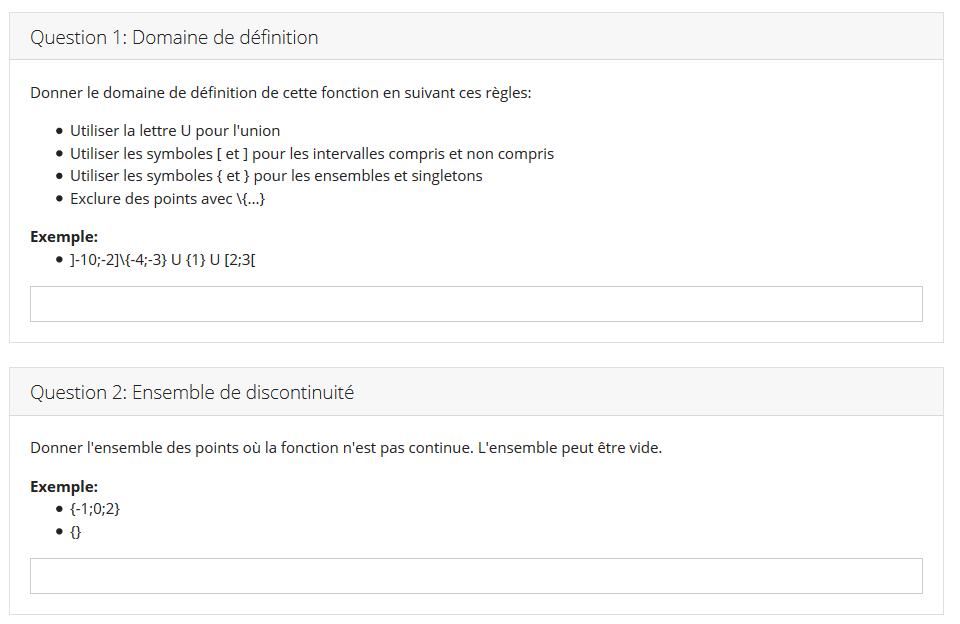
\includegraphics[scale=0.5]{images/dom.png}
\end{figure}

\newpage
\subsection{Coordonnées de point} \label{coord}

Cette section concerne les exercices demandant une réponse sous la forme de coordonnées de point comme (1.5,0) ou  (-5,2,10)
\bigskip

Les paramètres à modifier par rapport à un exercice simple sont les mêmes qu'au point précédent. C'est à dire qu'il faut laisser le "Grading environment type" sur "Docker container" et créer un sous-problème de type "code(une seule ligne)". 

La seule différence ce trouve dans l'onglet "Fichiers de l'exercice", où, après avoir créé un fichier nommé "run", vous devez copier le contenu du fichier "getCoordinates.py" présent ci-dessous ou disponible via ce lien : 

\bigskip
\url{https://github.com/UCL-INGI/inginious-math/blob/master/getCoordinates.py}
\bigskip

Collez-le ensuite dans le fichier "run" et modifiez-le en fonction des commentaires.

\lstinputlisting{codes/getCoordinates.py}

\bigskip

Voici un exemple d'exercice demandant des coordonnées de point :

\begin{figure}[!htb]
    \centering
    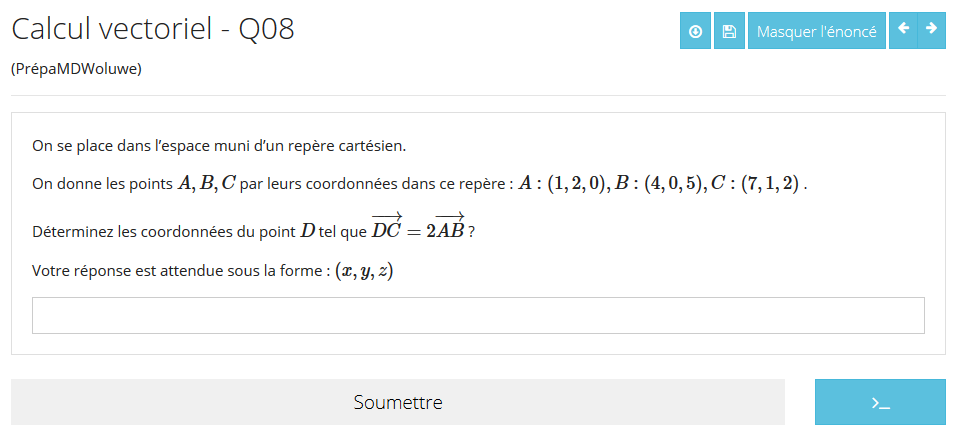
\includegraphics[scale=0.6]{images/coord.png}
\end{figure}

\newpage
\subsection{Paramètres random}\label{random}

Dans cette dernière partie nous allons expliquer comment réaliser un exercice comprenant des entrées générées aléatoirement (paramètres random). 
\bigskip

Par défaut les entrées sont différentes et fixes pour chaque étudiant, si vous souhaitez qu'elles changent à chaque rafraichissement de la page de l'exercice, indiquez le nombre de paramètres aléatoires dans l'onglet "Paramètres de base" et cochez la case "Regénérer l'entrée aléatoire" juste en dessous.
\bigskip

\begin{figure}[!htb]
    \centering
    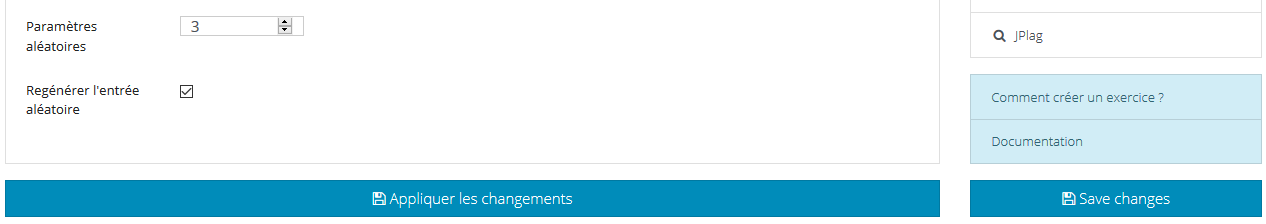
\includegraphics[scale=0.45]{images/Para_random.png}
\end{figure}


Concernant les paramètres, dans l'onglet "Environment", laissez le "Grading environment type" sur "Docker container" mais changez l'environnement de correction sur "math". 

Quand vous créez un sous-problème, sélectionnez le type "math". Dans l'énoncé de la question, écrivez :
\bigskip

.. raw${::}$ html

\bigskip
\hspace{1cm} Énoncé de la question. 

\bigskip
Quand il y a un nombre qui doit être généré aléatoirement, écrivez : \textbf{<b><span id="ipr1"></span></b>} avec l'id du paramètre que nous allons définir plus loin. 

Attention, les balises LaTeX ne fonctionnent pas dans le bloc html.

\bigskip

A la fin de la question, vous devez définir les paramètres aléatoires et leur id, vous êtes libre de choisir l'id et le nom de votre choix. Commencez par écrire ceci :
\bigskip

.. raw${::}$ html

\bigskip
\hspace{1cm} <script>

\bigskip
Ensuite, pour définir les variables, il faut faire comme ceci :
\bigskip

\hspace{2cm}var nom-de-la-variable =parseInt(input["@random"][indice] * 100);

\bigskip

Pour une variable aléatoire prise entre 0 et 100. L'indice doit être différent pour chaque variable et commencer à 0 (ex : 0,1,2,3...)

Attention il est important de respecter l'indentation !

\bigskip

Exemple de définition de variable:
\bigskip

\hspace{2cm}var somme = 10000*parseInt(input["@random"][0] * 100 + 1);

\hspace{2cm}var plus2 = 1000*parseInt(input["@random"][1] * 100 + 1);
\bigskip

Ici nous avons créé deux variables, un nombre est généré aléatoirement entre 0 et 100, on lui ajoute ensuite 1 et il est multiplié par 10000 pour la première variable, et 1000 pour la deuxième. Comme vous pouvez le constater, il est possible d'effectuer des opérations sur ces nombres afin qu'ils correspondent aux besoins de l'exercice.

\bigskip
Il faut ensuite définir l'id des variables comme ceci :
\bigskip

\hspace{2cm}document.getElementById("ID-choisi").innerHTML = nom-de-variable
\bigskip

L'id doit être différent pour chaque variable, et chaque variable doit posséder un id.

Exemple :
\bigskip

\hspace{2cm}document.getElementById("ipr1").innerHTML = somme;

\hspace{2cm}document.getElementById("ipr2").innerHTML = plus2;
\bigskip

Ici l'id de la variable "somme" a été défini comme étant "ipr1" et l'id de "plus2" comme étant "ipr2". Enfin, fermez le bloc par :
\bigskip

\hspace{1cm}</script>

\bigskip
Voici un exemple d'énoncé comprenant 3 entrées aléatoires :

\begin{figure}[!htb]
    \centering
    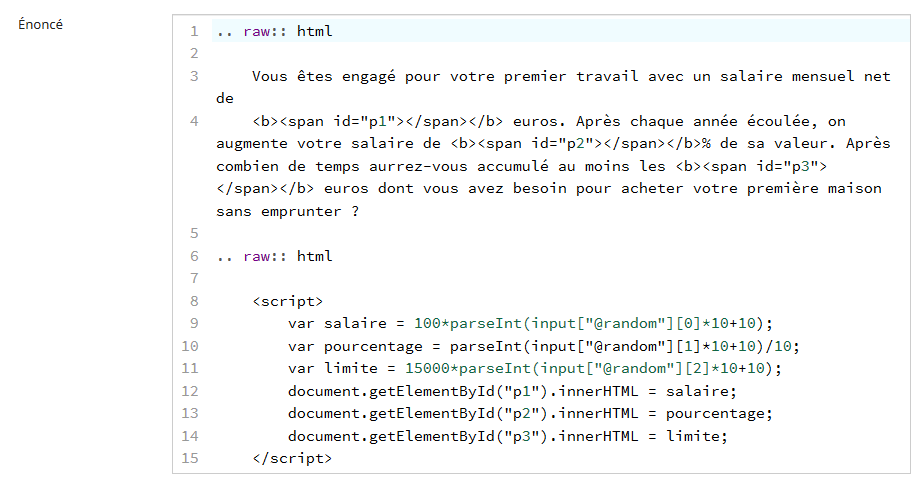
\includegraphics[scale=0.6]{images/random.png}
\end{figure}

Après avoir réalisé l'énoncé, ne rajoutez pas d'"Expected answer" et allez directement dans l'onglet "Fichiers de l'exercice" pour créer un fichier nommé "run". Copiez-collez ensuite le contenu du fichier "random.py" et modifiez votre fichier en suivant les commentaires. Le fichier est disponible via ce lien : 

\bigskip
\url{https://github.com/UCL-INGI/inginious-math/blob/master/random.py}
\bigskip

Et ci-dessous :

\newpage
\lstinputlisting{codes/random.py}

\section{Fonctionnalité supplémentaire}

\subsection{Graphe}

Il est possible d'intégrer des graphes dans les énoncés, ou même les feedbacks des exercices, ce qui est très utile pour représenter des fonctions ou des formes géométriques afin d'accompagner un problème.
\bigskip

Pour ce faire, qu'importe l'endroit où vous voulez que le graphe apparaisse, vous devez intégrer ceci à la \textbf{fin} de l'énoncé du sous-problème contenant un futur graphe :
\bigskip

.. raw${::}$ html
\bigskip

\hspace{1cm}<script type="text/javascript" charset="UTF-8" src="//jsxgraph.org/distrib/jsxgraphcore.js"></script>

\hspace{1cm}<link rel="stylesheet" type="text/css" href="//jsxgraph.org/distrib/jsxgraph.css" />
\bigskip

Attention à bien vérifier que la mise en page est respectée lorsque vous copiez-collez.
\bigskip

Une fois fait, vous allez pouvoir intégrer votre graphe à l'endroit désiré. En voici un exemple :
\bigskip

.. raw${::}$ html
\bigskip

\hspace{1cm}<div id={\color{red}'jxgbox1'} class='jxgbox mb-3' style='width:300px; height:150px;'></div>

\hspace{1cm}<script type='text/javascript'>

\hspace{2cm}var b = JXG.JSXGraph.initBoard({\color{red}'jxgbox1'}, {boundingbox: [-3, 3, 3, -2], axis: true});

\hspace{2cm}b.create('functiongraph', [function(x)\{return Math.cos(x);\},-2,2]);

\hspace{1cm}</script>
\bigskip

Vous pouvez modifier et ajouter des éléments à cet exemple pour qu'il corresponde à celui que vous désirez.

\begin{itemize}
    \item Modifier les valeurs de "height" et "width", qui sont exprimés en pixels, pour modifier la taille du cadre qui comprendra le graphe.
    \item Modifier les valeurs de "boundingbox" qui représente les coordonnées du coin supérieur gauche et du coin inférieur droit.
    \item Mettre "axis" à la valeur "false" pour faire disparaitre les axes du graphe.
    \item Remplacer "Math.cos(x)" par la fonction qui doit apparaitre sur le graphe. Exemple : 3*x**2 pour $\mathbf{3x^2}$
    \item Ajouter des lignes "b.create...." pour rajouter des fonctions sur le même graphe.
    \item Si plusieurs graphes dans une même question, il faut que l'id soit différent pour chaque graphe (en rouge dans l'exemple). L'id sert à différencier les graphes entre-eux.
\end{itemize}
\bigskip

Vous avez également la possibilité de rajouter des points, des lignes, des cercles et même des formes géométriques. Vous trouverez comment les réaliser via ce lien :
\bigskip

\url{https://jsxgraph.org/wiki/index.php/Documentation}

\bigskip

Voici un exemple d'énoncé, et le graphe qui lui correspond :

\begin{figure}[!htb]
    \centering
    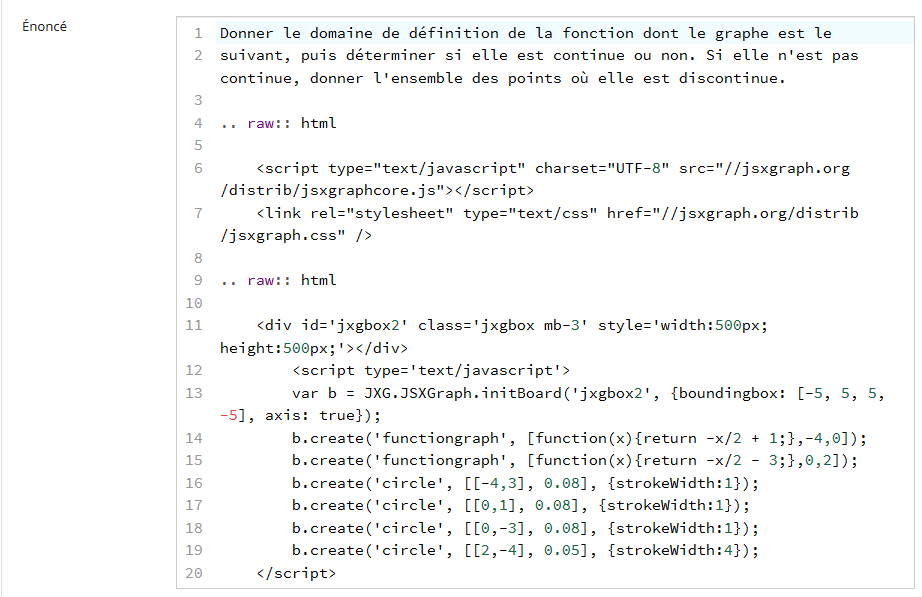
\includegraphics[scale=0.6]{images/fonc.png}
\end{figure}

\begin{figure}[!htb]
    \centering
    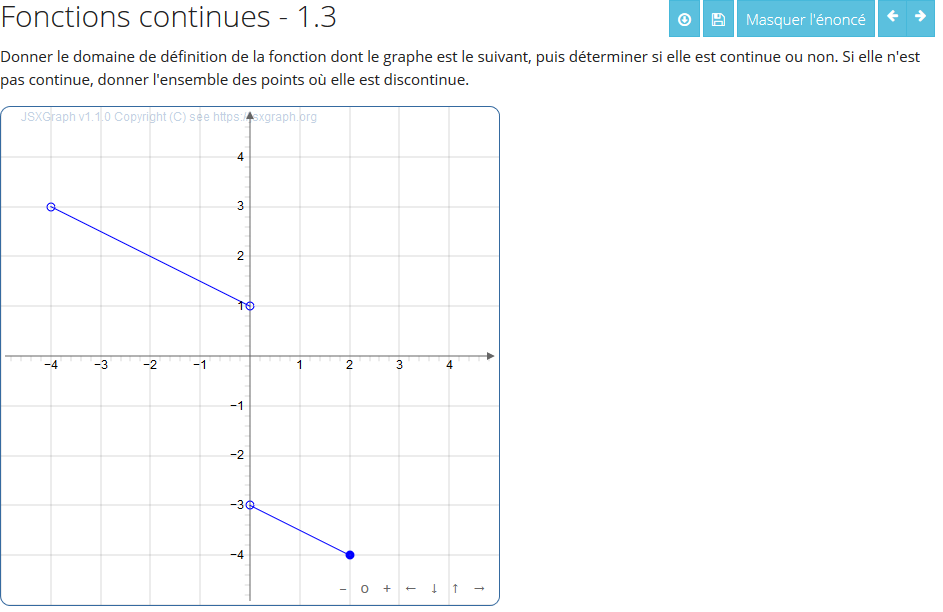
\includegraphics[scale=0.6]{images/graphe.png}
\end{figure}

















\end{document}
